\documentclass[12pt, a4paper]{article}

\usepackage{geometry}
\geometry{verbose,a4paper,tmargin=2cm,bmargin=2cm,lmargin=2cm,rmargin=2cm}
 
\usepackage[english]{babel}
\usepackage{amsmath}
\usepackage{mathtools}
\usepackage{cases}
\usepackage{hyperref}
\usepackage{longtable}
\usepackage{graphicx}
\graphicspath{ {../Media/} }

\title{SIR models for the spread of COVID-19}
\date{\today}
\author{
	Maksim Gordienko \\
	Alexander Sysoev
}

\begin{document}
	\maketitle
	
	\section{Introduction}
	In this article we are going to show how Kermack and McKendrick SIR models can be used for epidemic process simulation. Then we add vital dynamics to SIR model. Next we solve simple models in analytical way. Finally, we introduce sophisticated SEIRS-like model especially for COVID-19 conditions, close to real life.
	
	\section{Mathematical model of epidemics}
	Let's consider a group of $N$ people and classify them into these types:
	\begin{itemize}
		\item \textbf{S} -- Susceptible
		\item \textbf{I} -- Infected
		\item \textbf{R} -- Recovered
	\end{itemize}

	This is called the SIR model for the spread of epidemic diseases that describes the changes in numbers of the three types of individuals. We denote the number of susceptible persons by $s(t)$, the number of infected individuals by $i(t)$ and the number of recovered people by $r(t)$. The time $t$ is measured in days. Also we suppose that each person is in contact with $m$ persons per day average. Hence the number of contacts between the susceptible and infected people becomes $\frac{m}{N} i(t) s(t)$. If we set the probability of infection for each contact as $p$ then the number of newly infected individuals within $\Delta t$ days becomes
	\begin{equation}
		\frac{m}{N} i(t) s(t) p \Delta t
	\end{equation}
	in total. Let $\beta = mp$, the number of non-infected people \textbf{(S)} from the $t$-th day to $ (t + \Delta t) $-th day changes as
	\begin{equation}
		s(t + \Delta t) - s(t) = - \frac{\beta}{N} s(t) i(t) \Delta t
	\end{equation}
	When $\Delta t \rightarrow 0 $, we can rewrite it as differential equation
	\begin{equation}
		\frac{ds(t)}{dt} = - \frac{\beta}{N} s(t) i(t)
	\end{equation}
	Meanwhile, the infected individuals recover at a removal rate $ \gamma $ per day. Subsequently, increase in the number of the recovered persons becomes
	\begin{equation}
		\frac{dr(t)}{dt} = \gamma i(t)
	\end{equation}
	Respectively, $ \dfrac{1}{\gamma} $ is the expected duration of infection. Also the number of recovered people includes the amount of deceased persons because they cannot possibly infect others.
	
	\newpage
	
	As well as the total number of individuals is $N$, we can express $i(t)$
	\begin{equation}
		i(t) = N - s(t) - r(t)
	\end{equation}
	The change in the number of infected people can be written as
	\begin{equation}
		\frac{di(t)}{dt} = - \frac{ds(t)}{dt} - \frac{dr(t)}{dt} = \frac{\beta}{N} s(t) i(t) - \gamma i(t) = \frac{\beta}{N} (s(t) - \gamma) i(t)
	\end{equation}
	Gathering the equations above, we have
	\begin{numcases}{}
		\frac{ds(t)}{dt} = - \frac{\beta}{N} s(t) i(t) \label{eq:dsdt} \\
		\frac{di(t)}{dt} = (\frac{\beta}{N} s(t) - \gamma) i(t) \label{eq:didt} \\
		\frac{dr(t)}{dt} = \gamma i(t) \label{eq:drdt}
	\end{numcases}
	As initial conditions, we use
	\begin{equation} \label{eq:init_cond}
		\begin{dcases}
			s(0) = N_1 \\
			i(0) = N_2 \\
			r(0) = 0
		\end{dcases}
	\end{equation}
	If we introduce the following transformations of variables
	\[
		\tilde{s}(t) = \frac{s(t)}{N}, \tilde{i}(t) = \frac{i(t)}{N}, \tilde{r}(t) = \frac{r(t)}{N}, \tilde{t} = \beta t
	\]
	Then system of the equations becomes
	\begin{equation}
		\begin{dcases}
			\frac{d \tilde{s} (t)}{d \tilde{t}} = - \tilde{s}(t) \tilde{i}(t) \\
			\frac{d \tilde{i}(t)}{d \tilde{t}} = (\tilde{s}(t) - \frac{1}{R_0}) \tilde{i}(t) \\
			\frac{d \tilde{r}(t)}{d \tilde{t}} = \frac{1}{R_0} \tilde{i}(t)
		\end{dcases}
	\end{equation}
	The number $R_0 = \dfrac{\beta}{\gamma}$ is known as the basic reproduction number. The number of infected people increases when $R_0 > 1$ and decreases when $R_0 < 1$.
	
	\section{Analytical solution of SIR model}
	When model is defined, we can solve the system of equations \eqref{eq:dsdt} -- \eqref{eq:drdt}. For simplicity forget about function arguments. Firstly, rewrite the equation \eqref{eq:dsdt} as
	\begin{equation} \label{eq:dsdt_rewritten}
		i = - \frac{1}{\tilde{\beta}} (\frac{s'}{s})
	\end{equation}
	where $\tilde{\beta} = \dfrac{\beta}{N}$. Then differentiate both sides
	\begin{equation} \label{eq:di_1}
		i' = - \frac{1}{\tilde{\beta}} (- \frac{{s'}^2}{s^2} + \frac{s''}{s})
	\end{equation}
	Next insert the equation \eqref{eq:dsdt_rewritten} into \eqref{eq:didt}
	\begin{equation} \label{eq:di_2}
		i' = -(\tilde{\beta} s - \gamma) \frac{1}{\tilde{\beta}} (\frac{s'}{s})
	\end{equation}

	\newpage
	
	Comparing equations \eqref{eq:di_1} and \eqref{eq:di_2} we have
	\begin{equation} \label{eq:dsdt_combined}
		s \frac{d^2 s}{dt^2} - (\frac{ds}{dt})^2 + (\gamma - \tilde{\beta} s) s \frac{ds}{dt} = 0
	\end{equation}
	Now we introduce the following function
	\begin{equation} \label{eq:phi_intro}
		\phi = \frac{dt}{ds}
	\end{equation}
	Afterward \eqref{eq:dsdt_combined} becomes
	\begin{equation}
		\frac{d \phi}{ds} + \frac{\phi}{s} = (\gamma - \tilde{\beta} s)\phi^2
	\end{equation}
	This is a Bernoulli differential equation. Divide both parts by $ \phi^2 $
	\begin{equation}
		\frac{\phi'}{\phi^2} + \frac{1}{\phi s} = \gamma - \tilde{\beta} s
	\end{equation}
	Then make a substitution
	\begin{equation}
		z = \frac{1}{\phi}, z' = -\frac{\phi'}{\phi^2}
	\end{equation}
	Now solve the first-order linear ordinary equation
	\begin{equation}
		-z' + \frac{z}{s} = \gamma - \tilde{\beta} s 
	\end{equation}
	with general solution where $C$ is constant
	\begin{equation}
		z = -\gamma s \ln{s} + \tilde{\beta} s^2 + Cs
	\end{equation}
	Returning back to $\phi$
	\begin{equation} \label{eq:phi_res}
		\phi = \frac{1}{s(C - \gamma \ln{s} + \tilde{\beta} s)}
	\end{equation}
	From the relation of inverse function in equation \eqref{eq:phi_intro}, we have
	\begin{equation}
		\frac{1}{\phi} = \frac{ds}{dt}
	\end{equation}
	Using equation \eqref{eq:dsdt}, we obtain
	\begin{equation} \label{eq:it_def}
		i(t) = -\frac{1}{\tilde{\beta}} (C - \gamma \ln{s(t)} + \tilde{\beta} s(t))
	\end{equation}
	Moreover, from equations \eqref{eq:dsdt} and \eqref{eq:drdt}, we get
	\begin{equation}
		\frac{dr}{dt} = -\frac{\gamma}{\tilde{\beta}} (\frac{s'}{s})
	\end{equation}
	Subsequently, the relation between s(t) and r(t) becomes
	\begin{equation} \label{eq:rt_def}
		r(t) = -\frac{\gamma}{\tilde{\beta}} \ln{\frac{s(t)}{C_1}}
	\end{equation}
	where $C_1$ is a constant. According to our initial conditions \eqref{eq:init_cond} 
	\begin{equation}
		C_1 = N_1
	\end{equation}

	\newpage
	
	From the relation $s(0) + i(0) + r(0) = N$, we have
	\begin{equation}
		C = -\tilde{\beta}N + \gamma \ln{N_1}
	\end{equation}
	If we substitute $C$ into equation \eqref{eq:phi_res}, we obtain
	\begin{equation}
		\frac{dt}{ds} = \frac{1}{s(-\tilde{\beta}N - \gamma \ln{\dfrac{s}{N_1} + \tilde{\beta}s})}
	\end{equation}
	Integrate this and express $t$ as a function of $s$
	\begin{equation} \label{eq:t_eps}
		t = \int_{s(0)}^{s(t)} \frac{d \varepsilon}{\varepsilon(-\tilde{\beta}N - \gamma \ln{\dfrac{\varepsilon}{N_1}} + \tilde{\beta} \varepsilon)}
	\end{equation}
	For convenience, we change a variable
	\begin{equation}
		\xi = \frac{\varepsilon}{N_1}
	\end{equation}
	Rewrite the equation \eqref{eq:t_eps}
	\begin{equation}
		t(s) = \int_{1}^{\frac{s(t)}{N_1}} \frac{d \xi}{\xi(-\beta - \gamma \ln{\xi} + \beta \xi \frac{N_1}{N})}		
	\end{equation}
	Now we can calculate $t(s)$ using numerical integration with a small step size and $s(t)$ as a parameter like that
	\begin{equation}
		\int_{a}^{b} f(\xi) \,d\xi \simeq \sum_{i=0}^{n-1} f(a + ih)h,~ \text{where} ~ h = \frac{b-a}{n}
	\end{equation}
	If $t(s)$ is obtained, then $i(t)$ and $r(t)$ can be calculated from equations \eqref{eq:it_def} and \eqref{eq:rt_def} respectively.
	
	\newpage

	\section{SIR Model with natural deaths and births}

	Let's rewrite our system of equations \eqref{eq:dsdt} -- \eqref{eq:drdt} with an addition of the death and birth processes. Consider these rates are equal to each other, we introduce new variable $D$:
	\begin{numcases}{}
		\frac{ds(t)}{dt} = - \frac{\beta}{N} s(t) i(t) + D(N - s(t)) \label{eq:death_s} \\
		\frac{di(t)}{dt} = (\frac{\beta}{N} s(t) - \gamma - D) i(t) \label{eq:death_i} \\
		\frac{dr(t)}{dt} = \gamma i(t) - Dr(t) \label{eq:death_r}
	\end{numcases}
	As we did before, we rewrite it into one equation:
	\begin{equation} \label{eq:re_death_s}
		i = \frac{s' - D(N- s)}{-\tilde{\beta}s}
	\end{equation}
	Again we differentiate both sides (with $\tilde{\beta} = \frac{\beta}{N}$ substitution):
	\begin{equation}
		i' = -\frac{1}{\tilde{\beta}}(\frac{(s'' + D s')s - (s' + D s - D N)s'}{s^2}),
	\end{equation}
	\begin{equation} \label{eq:re_death_s_diff}	
		i' = -\frac{1}{\tilde{\beta}}(\frac{s''}{s} - \frac{s'^2 - D N s'}{s^2})
	\end{equation} 
	Now we can insert \eqref{eq:re_death_s} into \eqref{eq:death_i}:
	\begin{equation}
		i' = (\tilde{\beta} s - \gamma - D)(\frac{s' - D(N- s)}{-\tilde{\beta}s})
	\end{equation}
	\begin{equation} \label{eq:re_death_i_sub}
		i' = -\frac{1}{\tilde{\beta}s}(\tilde{\beta}s - \gamma - D)(s' + D s - D N)
	\end{equation}
	And comparing \eqref{eq:re_death_i_sub} and \eqref{eq:re_death_s_diff} we get next equation:
	\begin{equation} 
		s s'' - s'^2 +(-\tilde{\beta}s^2 + (\gamma + D)s + D N)s' - \tilde{\beta}D s^3 - (\tilde{\beta}D N + D(\gamma + D))s^2 - (\gamma + D)D N s = 0
	\end{equation}
	We can see that coefficients at $s^3, s^2$ and $s$ are $consts$ so we substitute them with \\ 
	$A = -\tilde{\beta}D, B = - (\tilde{\beta}D N + D(\gamma + D)),  C = - (\gamma + D)D N$:
	\begin{equation} \label{eq:death_main}
		s s'' - s'^2 +(-\tilde{\beta}s^2 + (\gamma + D)s + D N)s' +A s^3 + B s^2 + C s = 0
	\end{equation}
	Now we introduce a function $\phi = \frac{dt}{ds}$, so the equation will be:
	\begin{equation} \label{eq:death_main_phi}
		-\phi' - \frac{\phi}{s} +(-\tilde{\beta}s^2 + (\gamma + D)s + D N)\frac{\phi^2}{s} + (A s^2 + B s + C)\phi^3 = 0
	\end{equation}
	And by substitution $v = \phi s, v' = \phi's + \phi$ the following equation occur:
	\begin{equation} \label{eq:death_main_v}
		v' +(-\tilde{\beta} + \frac{(\gamma + D)}{s} + \frac{D N}{s^2})v^2 + (A + \frac{B}{s} + \frac{C}{s^2})v^3 = 0
	\end{equation}

	\newpage
	Then we assume these three substitutions:
	\begin{numcases}{}
		r(s) = \frac{1}{v(s)}, \\
		\xi(s) = (\tilde{\beta} - \frac{(\gamma + D)}{s} - \frac{D N}{s^2}), \\
		\eta(s) = -(A + \frac{B}{s} + \frac{C}{s^2})
	\end{numcases}
	and we get Abel-type first-order second-kind equation:
	\begin{equation}
		r r' = \xi(s)r + \eta(s)
	\end{equation}

	\newpage
	
	\section{Modeling COVID-19 pandemic}

	\subsection{Definitions}

	In order to create lifelike COVID-19 infection model we need to introduce more parameters in our model and consider different spread cases.
	\begin{itemize}
		\item \textbf{$S$} -- Susceptible. Includes all individuals who are not infected but are susceptible to contract the disease.
		\item \textbf{$E$} -- Exposed. Includes all persons who are exposed to infection, but not yet infections. Some of them might fall ill and some may not. We introduced that component due to incubation period of COVID-19 pandemic (approximated 5-6 days by WHO).
		\item \textbf{$I_s$} -- Symptomatic infected. It includes all the individuals who were symptomatic and infectious. They have approached some health-care facility, but have not yet been quarantined. This compartment was brought into the picture considering concerning news from worst-affected counties like Italy and the U.S. of the hospitals and health-care centers getting filled up very fast during this pandemic. A significant portion of the infected individuals may not be quarantined in case of the health-care system collapses.
		\item \textbf{$I_{as}$} -- Asymptomatic infected. It includes all those people who are affected but asymptomatic before they either recover or die or get permanently disabled. This compartment was formalized keeping after reports of various authentic studies claiming that around 30-40 percent of the infected individuals remain
		asymptomatic.
		\item \textbf{$Q$} -- Quarantined. Includes all persons who are currently under quarantine in healh-care facility.
		\item \textbf{$Q'$} -- In intensive care unit. Includes the quarantined patients who had to be moved to ICU after their condition worsened.
		
		\item \textbf{$C$} -- Carrier. This compartment includes individuals who have left quarantine after being tested negative but actually have not fully healed. So they can possibly infetct other susceptible individuals. They eventually either fall sick again or recover from disease. We introduced it due to multiple cases of re-infection being reported from countries like South Korea, China and Japan. It is safe to assume that one of the following happened:
		\begin{enumerate}
			\item Medical inefficiency (inaccurate test result)
			\item Loss of immunity after recovery and subsequent re-infection
		\end{enumerate}
		For the first possibility we introduced the $C$ compartment. To account for the second possibility we have kept the transition from $R$ to $S$ compartment respectively.
		\item $R_{wd}$ -- Recovered without disability. It includes all individuals who have recovered from infection without any disability and they can no longer infect any other individual
		\item $D$ -- Deceased. Includes all deaths during the pandemic.
		\item $R_d$ -- Recovered with disability. In this compartment we have kept all people who have recovered from the infection, can no longer infect anyone else but have been permanently disabled post recovery.
	\end{itemize}
	 
	\newpage

	\subsection{Formualting differential equations}

	Now we can define differential equations corresponding to described model above.

	\begin{equation}
		\frac{dS}{dt} = -\alpha \frac{S(I_s + I_{as} + C)}{N} + g R_{wd}
	\end{equation}
	Where $\alpha$ is the disease transmission rate (same as $\beta = mp$ in SIR model) and $g$ is the rate at which a fraction of recovered individuals lose their immunity.

	\begin{equation}
		\frac{dE}{dt} = \alpha \frac{S(I_s + I_{as} + C)}{N} - \mu E
	\end{equation}
	If average incubation period is taken to be an exponential distribution $\mu$.

	\begin{equation}
		\frac{d I_s}{dt} = r \mu E - \varepsilon I_s + fC - \zeta_1 I_s - \eta_1 I_s
	\end{equation}
	Where $f$ is rate at which a fraction of carriers gets re-infected. Here $0 \le r \le 1$ is a number which shows how many individuals in the exposed compartment moves to $I_s$ compartment rather than $I_{as}$ one. And $\varepsilon, \zeta_1, \eta_1$ are the rates at which infected individuals get quarantined, deceased, disabled respectively.

	\begin{equation}
		\frac{d I_{as}}{dt} = (1 - r)\mu E - \beta_3 I_{as} - \zeta_3 I_{as} - \eta_3 I_{as}
	\end{equation}
	Where $\beta_3, \zeta_3$ and $\eta_3$ are the recovery rate, death rate and disability rate of asymptomatic individuals respectively.

	\begin{equation}
		\frac{dQ}{dt} = \varepsilon I_s - \beta_1 Q - vQ - pQ - \zeta_2 Q - \eta_2 Q
	\end{equation}
	Where $v, p, \zeta_2$ and $\eta_2$ are the rates at which the quarantined individuals go to carrier state, ICU, deceased and disabled compartments respectively. $\beta_1$ is the recovery rate for quarantined people.
	
	\begin{equation}
		\frac{d Q'}{dt} = pQ - \beta_4 Q' - \zeta_5 Q' - \eta_5 Q'
	\end{equation}
	Where $\beta_4, \zeta_5$ and $\eta_5$ are the rate with which individuals in ICU recover, die and get disabled respectively.

	\begin{equation}
		\frac{dC}{dt} = vQ - fC - \beta_2 C - \zeta_4 C - \eta_4 C
	\end{equation}
	Where $\beta_2, \zeta_4$ and $\eta_4$ are the rate with which carrier individuals recover, die and get disabled silently, respectively.

	\begin{equation}
		\frac{dR_{wd}}{dt} = \beta_1 Q + \beta_3 I_{as} + \beta_2 C - gR_{wd}
	\end{equation}

	\begin{equation}
		\frac{dD}{dt} = \zeta_1 I_s + \zeta_2 Q + \zeta_3 I_{as} + \zeta_4 C + \zeta_5 Q'
	\end{equation}

	\begin{equation}
		\frac{dR_d}{dt} = \eta_1 I_s + \eta_2 Q + \eta_3 I_{as} + \eta_4 C + \eta_5 Q'
	\end{equation}

	System of these equations can be solved using numerical methods.

	\newpage

	\subsection{Parameters and initial conditions selection}

	\begin{longtable}[c]{| c | c | c | c | c | c |}
		\caption{Initial condtions and rates}\\
		\hline
		Initial condition & Value & Rate & Value & Rate & Value\\
		\hline
		$N$ & 83783945 & $\alpha$ & 0.42 & $v$ & 0.05 \\
		$S$ & 83783845 & $g$ & 0.0001 & $p$ & 0.01\\
		$E$ & 0 & $\mu$ & 7 & $\zeta_2$ & 0.2\\
		$I_s$ & 100 & $f$ & 0.2 & $\eta_2$ & 0.1 \\
		$I_{as}$ & 0 & $r$ & 0.3 & $\beta_1$ & 0.5\\
		$Q$ & 0 &$\varepsilon$ & 0.5 & $\beta_4$ & 0.05\\
		$Q'$ & 0 &$\zeta_1$ & 0.025 & $\zeta_5$ & 0.2 \\
		$C$ & 0 &$\eta_1$ & 0.1 & $\eta_5$ & 0.1\\
		$R_{wd}$ & 0 & $\beta_3$ & 0.1458 & $\beta_2$ & 0.1458\\
		$D$ & 0 & $\zeta_3$ & 0.1 & $\zeta_4$ & 0.05\\
		$R_d$ & 0 & $\eta_3$ & 0.05 & $\eta_4$ & 0.01\\
		\hline

	\end{longtable}

	We decided to use early data from Germany for modeling epidemics. Data sources links provided at the end of article. Primarily, we relied on dataset by \textit{Our World in Data}. Rates were calculated using correlation with recent observations, research news and publications. These values were actual on February 2, 2020. We take into account further statistics to fine tune the parameters closer to real life.

	\subsection{Obtained results}

	\begin{figure}[h!]
		\centering
		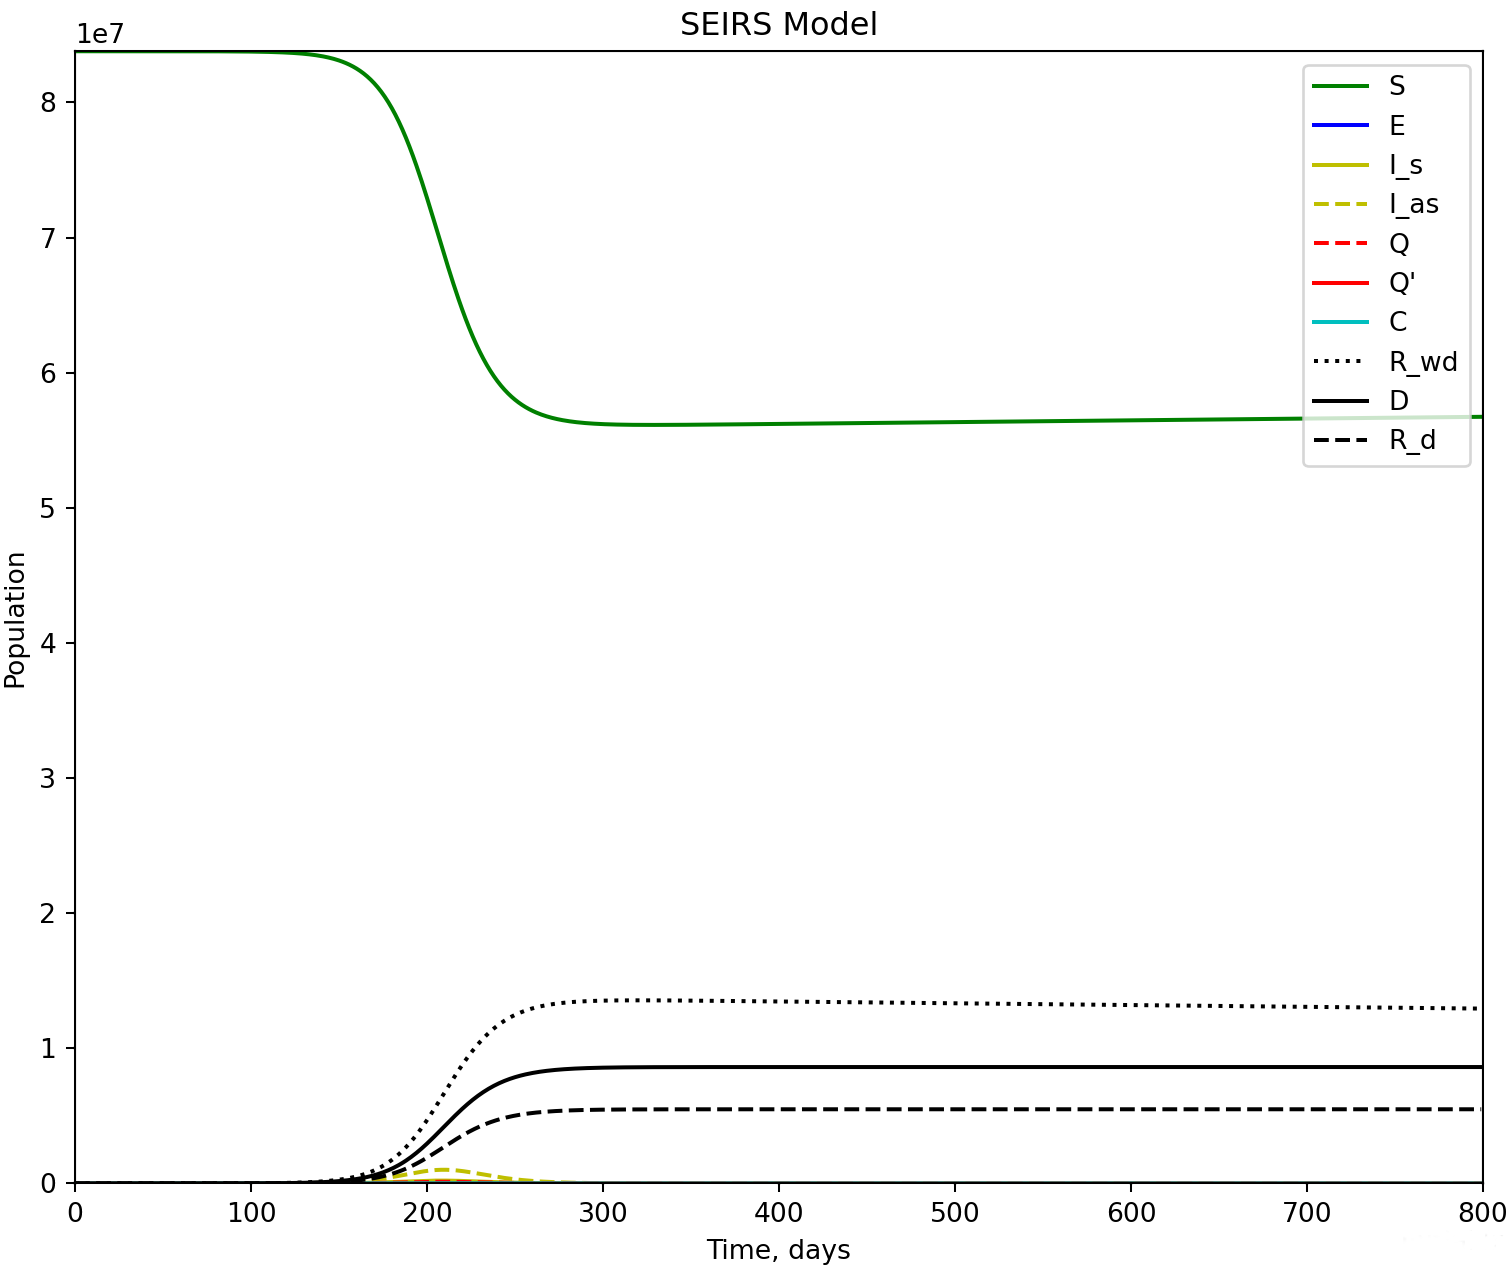
\includegraphics[width=12cm]{seirs.png}
		\caption{SEIRS model with fixed disease transmission rate $\alpha = 0.42$.}
	\end{figure}

	\newpage

	\begin{figure}[h!]
		\centering
		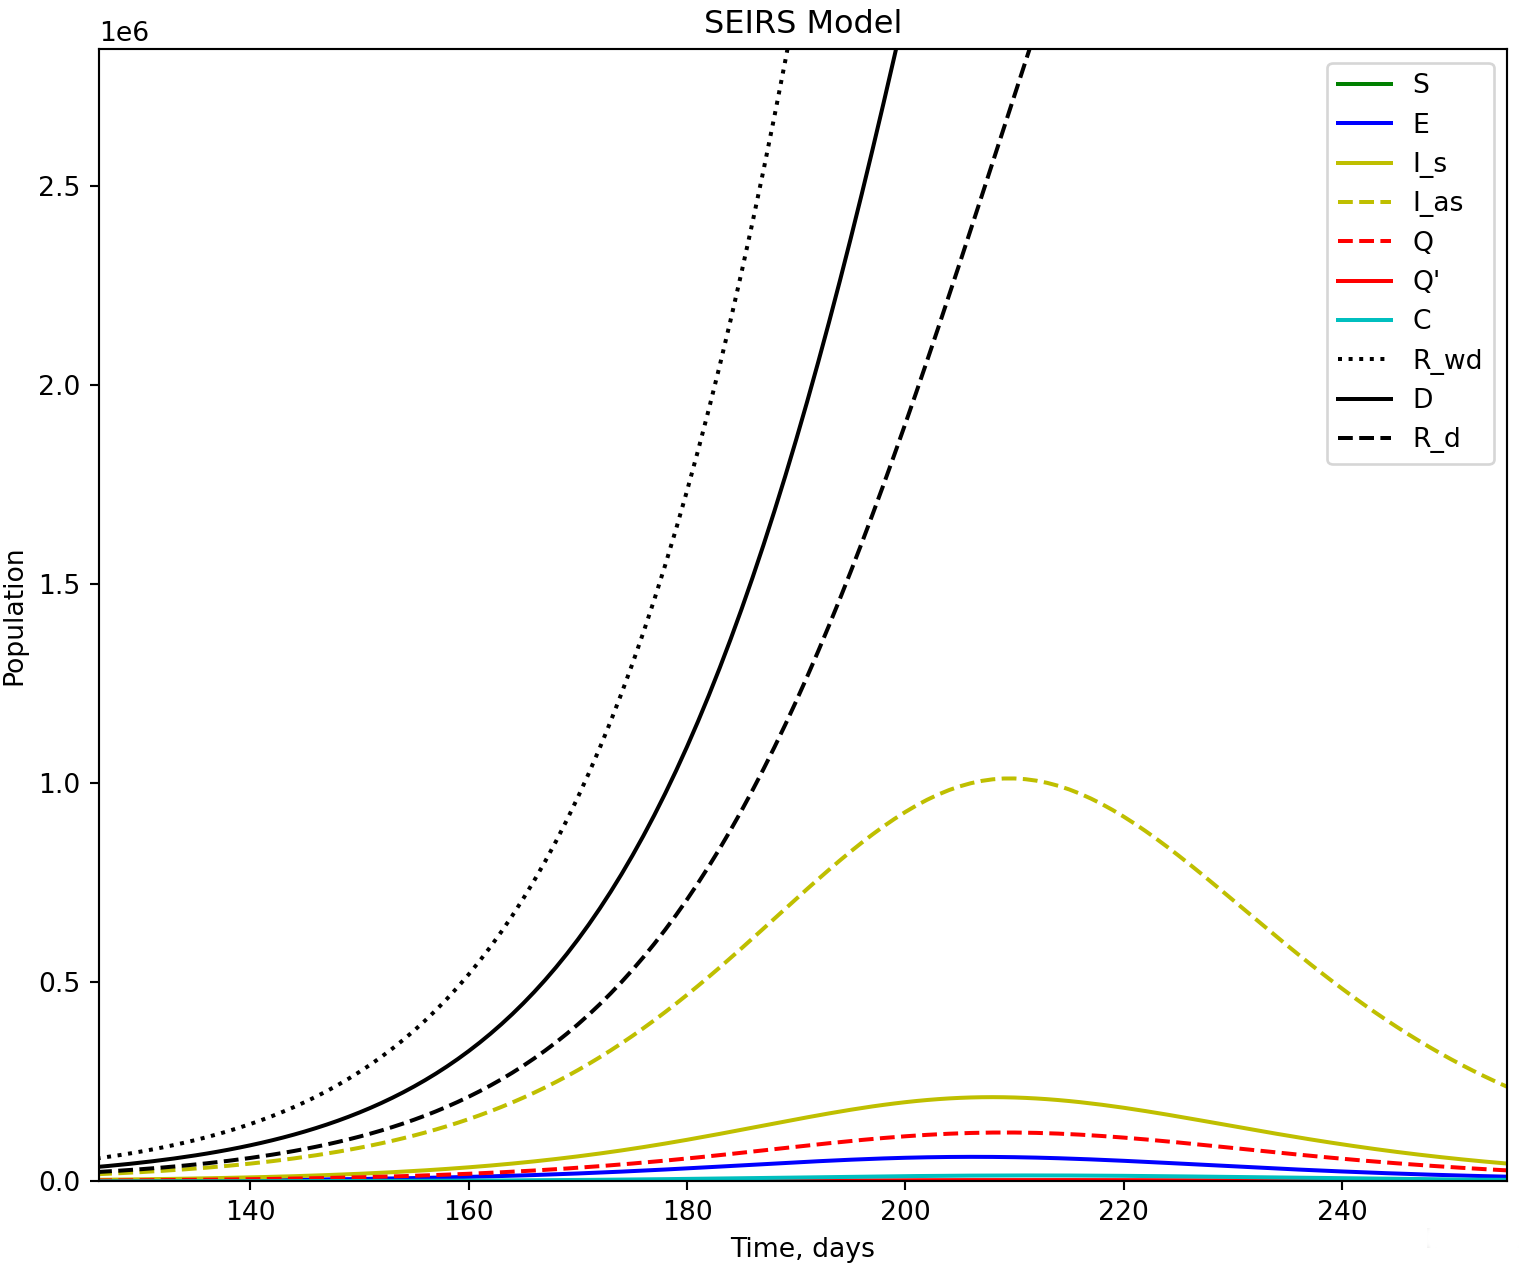
\includegraphics[width=12cm]{seirs_2.png}
		\caption{SEIRS model with fixed disease transmission rate $\alpha = 0.42$. Zoomed to outbreak.}
	\end{figure}

	Let's see how conditions getting worse if people simply do not maintain social distance and neglet personal protective equipment like masks. Potentially number of contacts and probability of getiing infection increases as well as our $\alpha$ rate.

	\begin{figure}[h!]
		\centering
		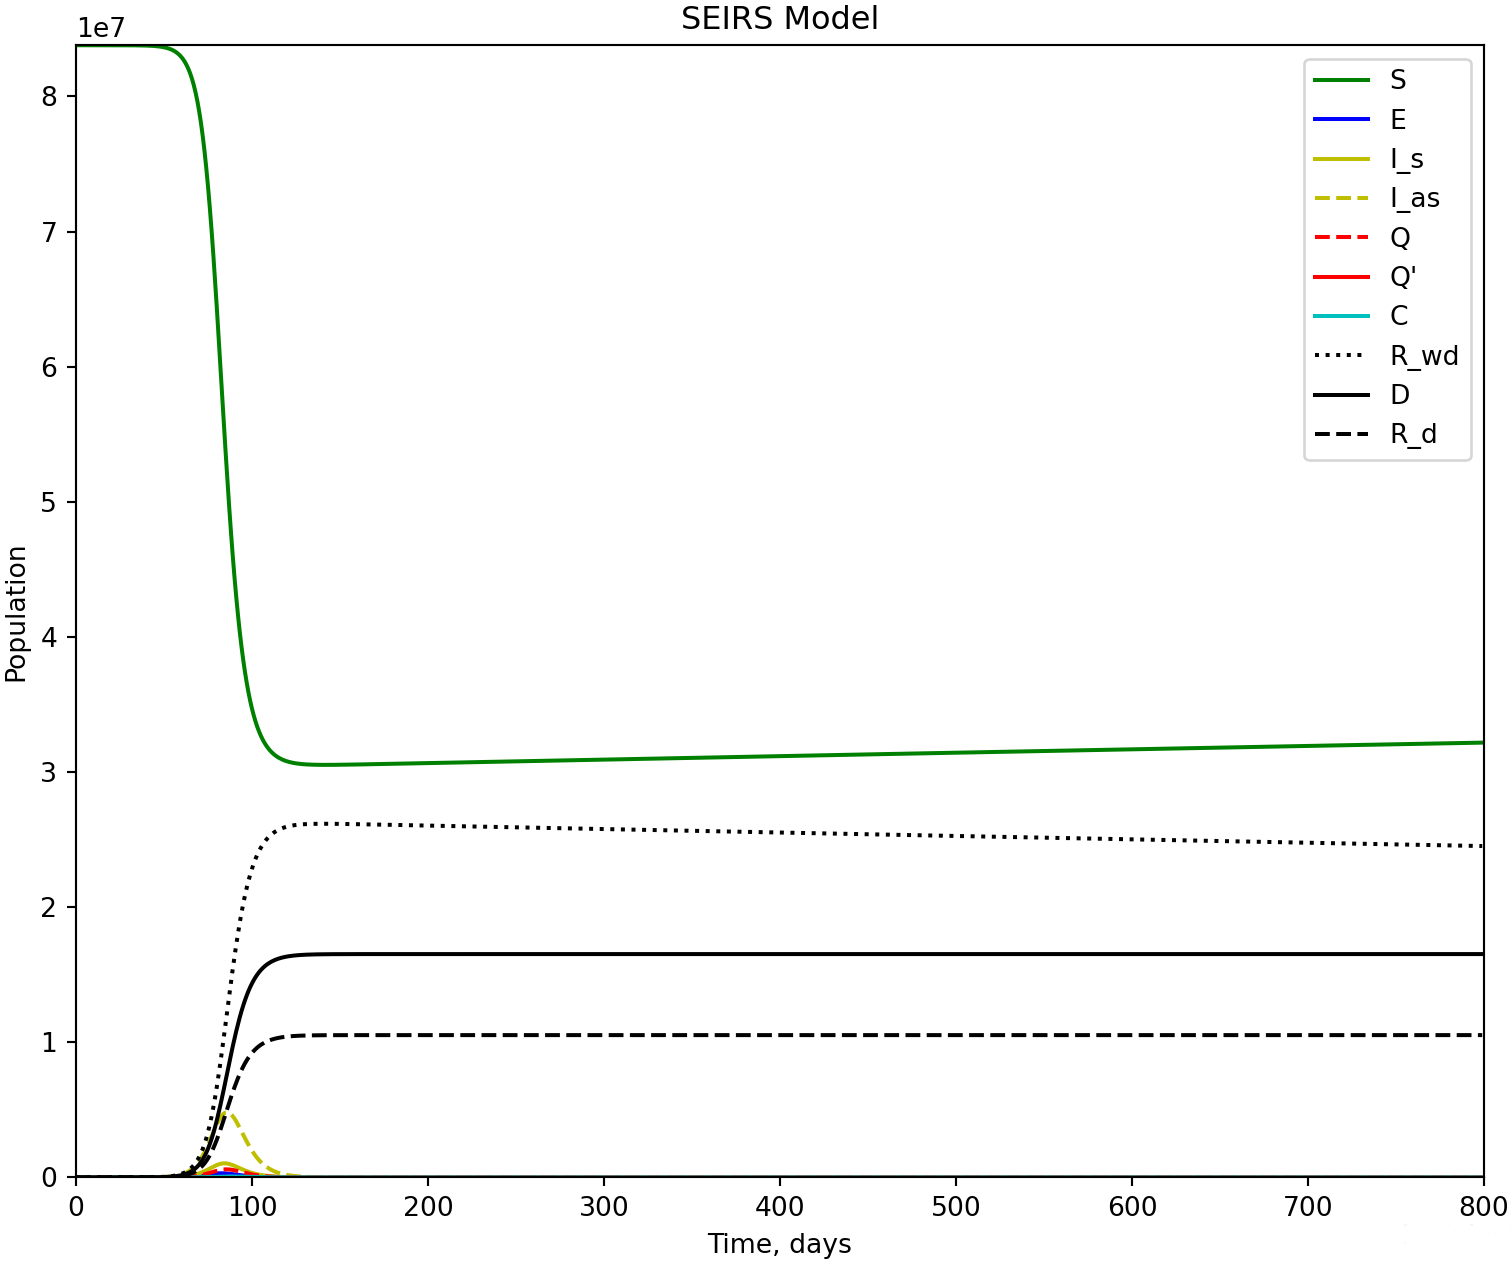
\includegraphics[width=12cm]{seirs_bigalpha.png}
		\caption{SEIRS model with increased $\alpha = 0.55$.}
	\end{figure}

	\newpage

	\begin{figure}[h!]
		\centering
		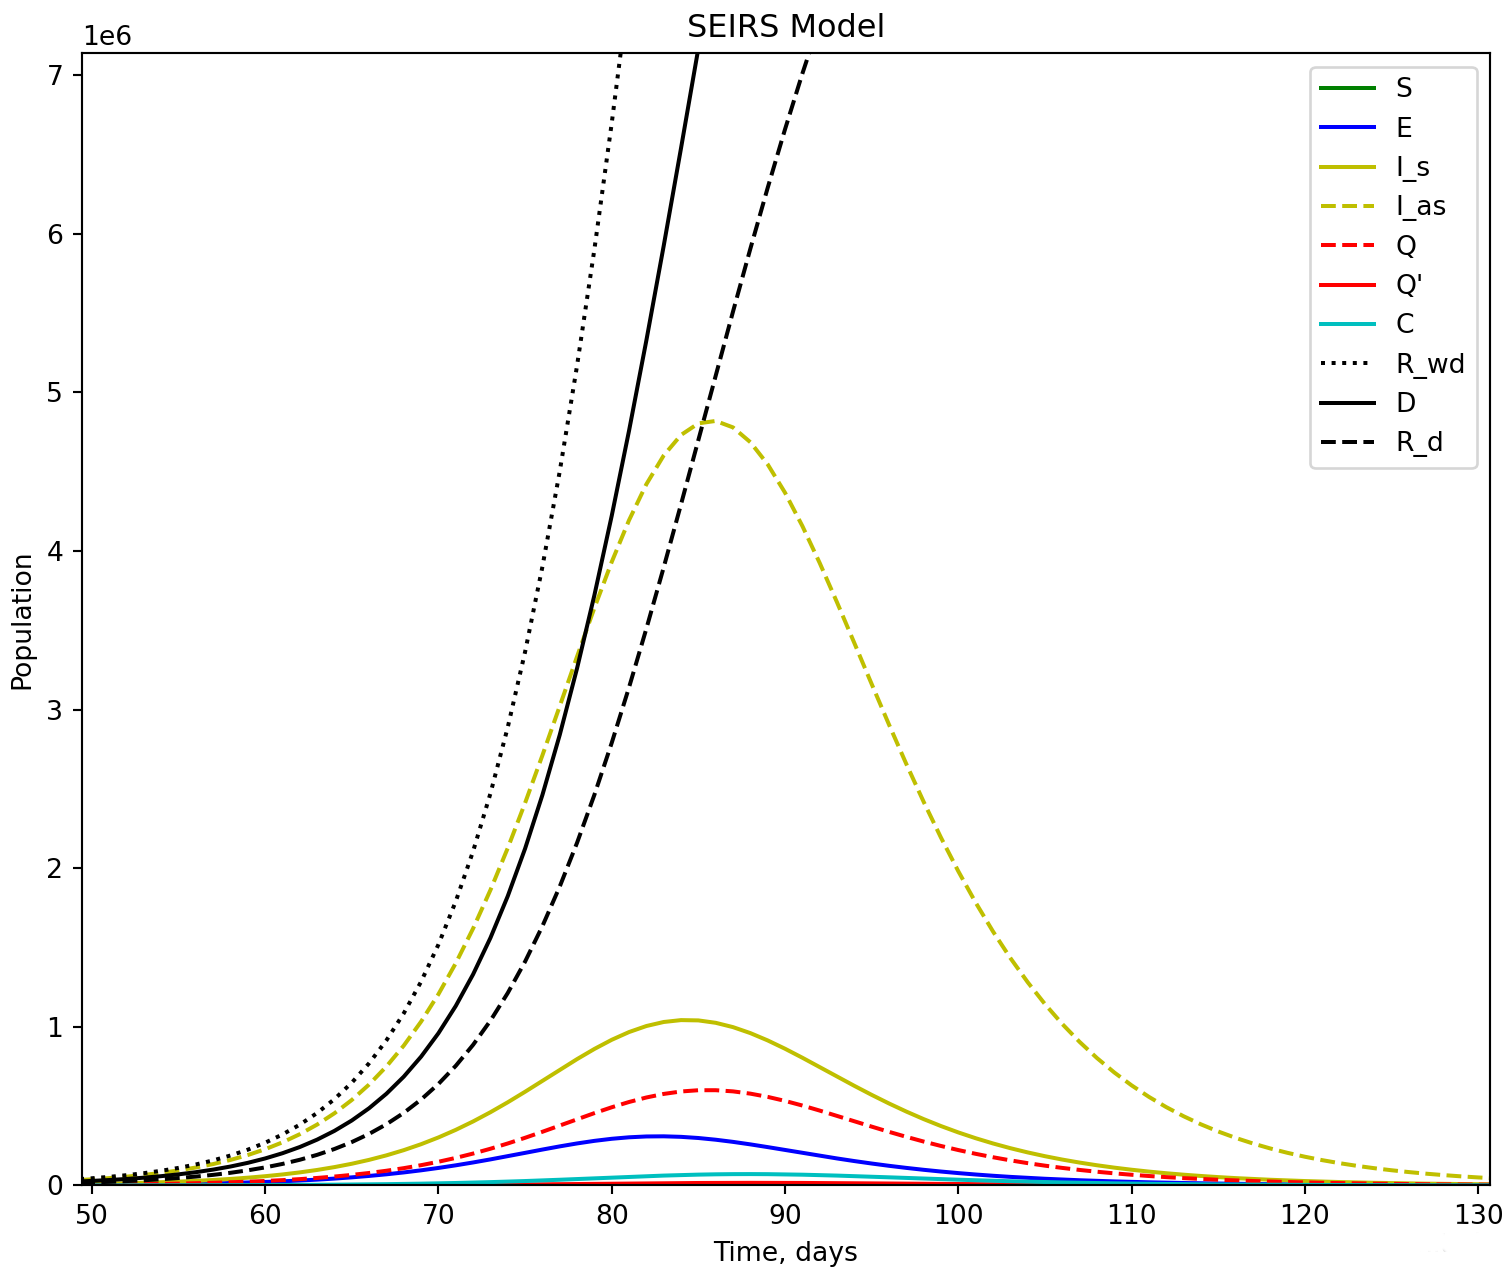
\includegraphics[width=12cm]{seirs_bigalpha_2.png}
		\caption{SEIRS model with increased $\alpha = 0.55$. Zoomed to outbreak.}
	\end{figure}

	We observe that expected outbreak occured earlier. Number of asymptomatic infected people reaches 5 millon, comparing with about 1 millon before. Meanwhile, the amount of deaths has almost doubled. Rapidly decreasing susceptible people means the high rate of infection. Thus, the situation has greately worsened. It means a heavy burden on medical institutions and will affect every aspect of our life.

	\section{References and data sources}

	\begin{itemize}
		\item Exact analytical solutions of the Susceptible-Infected-Recovered (SIR) epidemic
		model and of the SIR model with equal death and birth rates. Tiberiu Harko, Francisco S. N. Lobo, M. K. Mak.

		\item A Mathematical Model of Epidemics—A Tutorial
		for Students. Yutaka Okabe and Akira Shudo. Department of Physics, Tokyo Metropolitan University, Hachioji, Tokyo 192-0397, Japan.

		\item Modelling and simulation of COVID-19 propagation in a large population with specific reference to India.
		Ashish Menon, Nithin K Rajendran, Anish Chandrachud, Girish Setlur. Department of Physics, Indian Institute of Technology Guwahati.

		\item Statistics of the COVID-19 pandemic in Germany: \url{https://en.wikipedia.org/wiki/Statistics_of_the_COVID-19_pandemic_in_Germany}
	
		\item Close to 17 percent of patients recovered from COVID-19 could still carry virus: \url{https://www.sciencedaily.com/releases/2020/10/201028134029.htm}
		
		\item Flattening the disability curve: Rehabilitation and recovery after COVID-19 infection: \url{https://www.ncbi.nlm.nih.gov/pmc/articles/PMC7211743/}
		
		\item Complete COVID-19 dataset maintained by Our World in Data: \url{https://github.com/owid/covid-19-data/tree/master/public/data/}
	\end{itemize}
\end{document}